\setlength{\columnsep}{3pt}
\begin{flushleft}

	\begin{itemize}
		\item List all the available zones:
		\begin{tcolorbox}[breakable,notitle,boxrule=1pt,colback=pink,colframe=pink]
			\color{black}
			\fontdimen2\font=1em
			Syntax: firewall-cmd --get-zones
			\fontdimen2\font=4pt
		\end{tcolorbox}	
		Eg:
		\begin{figure}[h!]
			\centering
			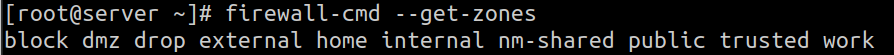
\includegraphics[scale=0.4]{content/chapter2/images/zones.png}
			\caption{Sample output}
			\label{fig:zones}
		\end{figure}
		
		\bigskip
		\bigskip
		
		\item Display the default zones:
		\begin{tcolorbox}[breakable,notitle,boxrule=1pt,colback=pink,colframe=pink]
			\color{black}
			\fontdimen2\font=1em
			Syntax: firewall-cmd --get-default-zone
			\fontdimen2\font=4pt
		\end{tcolorbox}	
		Eg:
		\begin{figure}[h!]
			\centering
			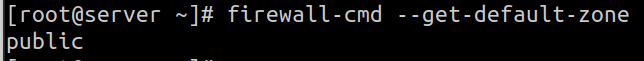
\includegraphics[scale=0.5]{content/chapter2/images/zones2.png}
			\caption{Sample output}
			\label{fig:zones2}
		\end{figure}

		\bigskip
		\bigskip

		\item Set the default zone:
		\begin{tcolorbox}[breakable,notitle,boxrule=1pt,colback=pink,colframe=pink]
			\color{black}
			\fontdimen2\font=1em
			Syntax: firewall-cmd --set-default-zone=<zone>
			\fontdimen2\font=4pt
		\end{tcolorbox}	
		Eg:
		\begin{figure}[h!]
			\centering
			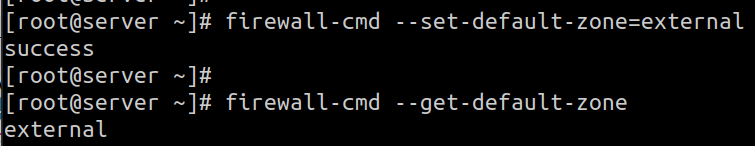
\includegraphics[scale=0.45]{content/chapter2/images/zones3.png}
			\caption{Sample output}
			\label{fig:zones3}
		\end{figure}

		\newpage

		\item Display information for all zones (interfaces, sources, ports, services, etc).
		\bigskip
		\begin{tcolorbox}[breakable,notitle,boxrule=1pt,colback=pink,colframe=pink]
			\color{black}
			\fontdimen2\font=1em
			Syntax: firewall-cmd ---list-all-zones
			\fontdimen2\font=4pt
		\end{tcolorbox}	

		\bigskip
		\bigskip		
		
		\item Display information for specific zone (interfaces, sources, ports, services, etc). If no \textbf{"--zone="} option is provided, the default zone will be used.
		\bigskip
		\begin{tcolorbox}[breakable,notitle,boxrule=1pt,colback=pink,colframe=pink]
			\color{black}
			\fontdimen2\font=1em
			Syntax: firewall-cmd ---list-all [--zone=<ZONE>]
			\fontdimen2\font=4pt
		\end{tcolorbox}	
		Eg:
		\begin{figure}[h!]
			\centering
			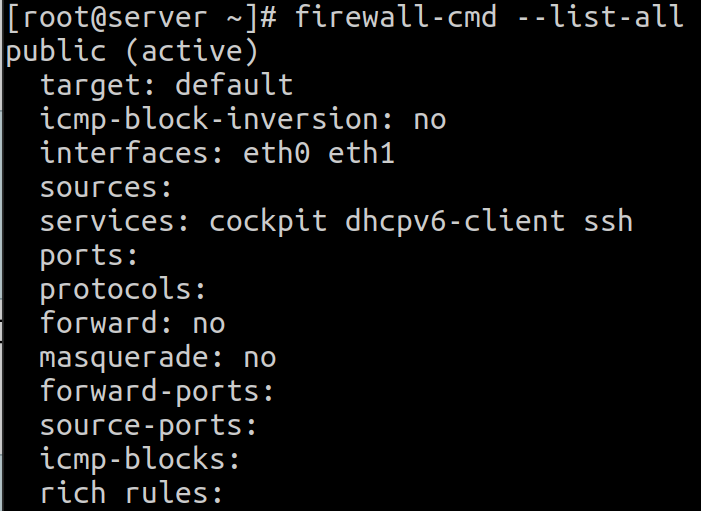
\includegraphics[scale=0.4]{content/chapter2/images/zones5.png}
			\caption{Sample output}
			\label{fig:zones4}
		\end{figure}

		\newpage
		\item Apply changes done by \textbf{firewall-cmd} command immediately:
		\begin{tcolorbox}[breakable,notitle,boxrule=1pt,colback=pink,colframe=pink]
			\color{black}
			\fontdimen2\font=1em
			Syntax: firewall-cmd ---reload
			\fontdimen2\font=4pt
		\end{tcolorbox}	
		
		\bigskip
		\bigskip
		
		\item Allow traffic to <SERVICE>. If no --zone= option is provided, the default zone will be used.
		\bigskip
		\begin{tcolorbox}[breakable,notitle,boxrule=1pt,colback=pink,colframe=pink]
			\color{black}
			\fontdimen2\font=1em
			Syntax: 
			\newline
			firewall-cmd ---add-service=<service> ---permanent [--zone=<ZONE>]
			\newline
			\newline
			firewall-cmd ---reload
			\fontdimen2\font=4pt
		\end{tcolorbox}	
		Eg:
		\begin{tcolorbox}[breakable,notitle,boxrule=-0pt,colback=black,colframe=black]
			\color{green}
			\fontdimen2\font=1em
			\# firewall-cmd --add-service=httpd --permanent 
			\newline
			\# firewall-cmd --reload
			\fontdimen2\font=4pt
		\end{tcolorbox}
		\begin{figure}[h!]
			\centering
			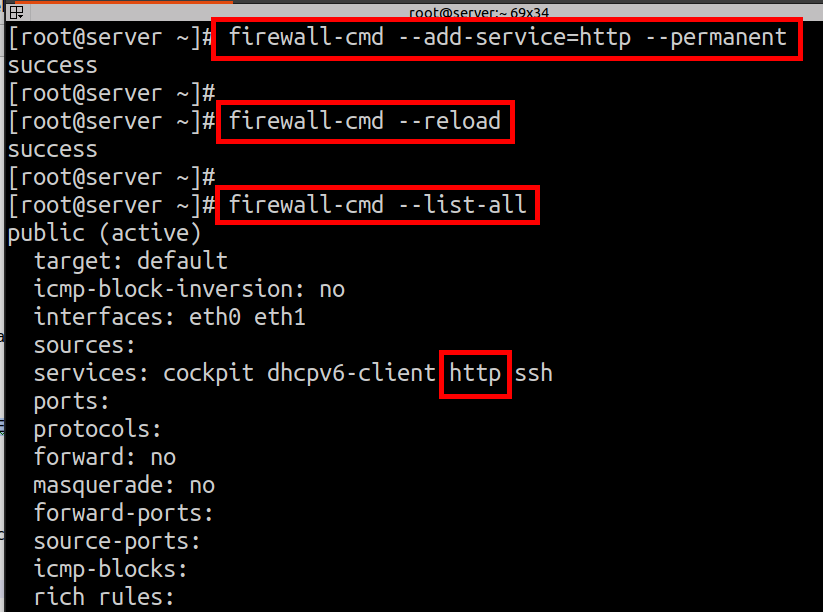
\includegraphics[scale=0.4]{content/chapter2/images/zones6.png}
			\caption{Sample output}
			\label{fig:zones6}
		\end{figure}
		\newpage
		
		\item Remove <SERVICE> from the allowed list for the zone. If no \textbf{"--zone="} option is provided, the default zone will be used.
		\bigskip
		\begin{tcolorbox}[breakable,notitle,boxrule=1pt,colback=pink,colframe=pink]
			\color{black}
			\fontdimen2\font=1em
			Syntax: 
			\newline
			firewall-cmd ---remove-service=<service> ---permanent [--zone=<ZONE>]
			\newline
			\newline
			firewall-cmd ---reload
			\fontdimen2\font=4pt
		\end{tcolorbox}	
		Eg:
		\begin{tcolorbox}[breakable,notitle,boxrule=-0pt,colback=black,colframe=black]
			\color{green}
			\fontdimen2\font=1em
			\# firewall-cmd --remove-service=httpd --permanent 
			\newline
			\# firewall-cmd --reload
			\fontdimen2\font=4pt
		\end{tcolorbox}
		\begin{figure}[h!]
			\centering
			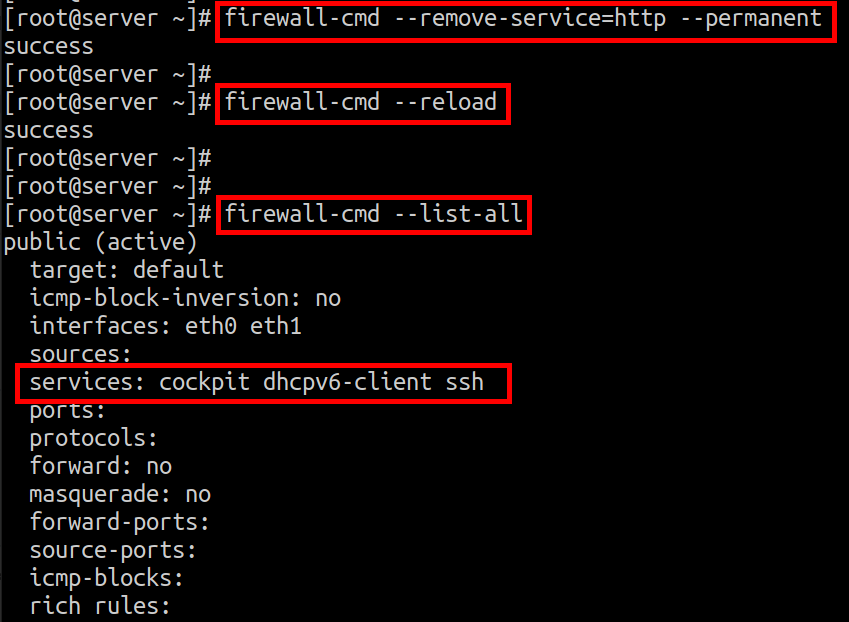
\includegraphics[scale=0.4]{content/chapter2/images/zones7.png}
			\caption{Sample output}
			\label{fig:zones7}
		\end{figure}
		
		\newpage
		\item Allow traffic to the \textbf{<PORT/PROTOCOL>} port(s). If no \textbf{"--zone="} option is provided, the default zone will be used.
		\bigskip
		\begin{tcolorbox}[breakable,notitle,boxrule=1pt,colback=pink,colframe=pink]
			\color{black}
			\fontdimen2\font=1em
			Syntax: 
			\newline
			firewall-cmd ---add-port=<PORT/PROTOCOL> ---permanent [--zone=<ZONE>]
			\newline
			\newline
			firewall-cmd ---reload
			\fontdimen2\font=4pt
		\end{tcolorbox}	
		Eg:
		\begin{tcolorbox}[breakable,notitle,boxrule=-0pt,colback=black,colframe=black]
			\color{green}
			\fontdimen2\font=1em
			\# firewall-cmd --add-port=6060/tcp --permanent 
			\newline
			\# firewall-cmd --reload
			\fontdimen2\font=4pt
		\end{tcolorbox}
		\begin{figure}[h!]
			\centering
			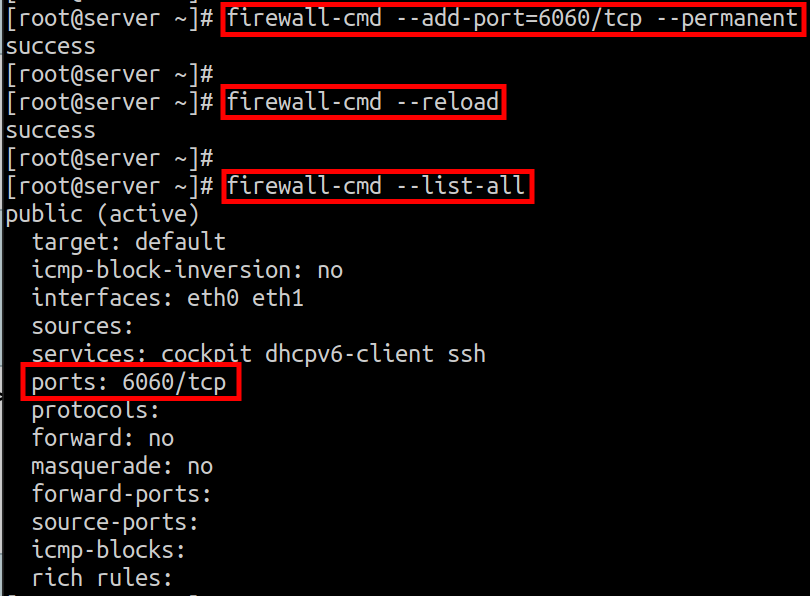
\includegraphics[scale=0.4]{content/chapter2/images/zones8.png}
			\caption{Sample output}
			\label{fig:zones8}
		\end{figure}
		
		\newpage
		\item Remove the <PORT/PROTOCOL> port(s) from the allowed list for the zone. If no \textbf{"--zone="} option is provided, the default zone will be used.
		\bigskip
		\begin{tcolorbox}[breakable,notitle,boxrule=1pt,colback=pink,colframe=pink]
			\color{black}
			\fontdimen2\font=1em
			Syntax: 
			\newline
			firewall-cmd ---remove-port=<PORT/PROTOCOL> ---permanent [--zone=<ZONE>]
			\newline
			\newline
			firewall-cmd ---reload
			\fontdimen2\font=4pt
		\end{tcolorbox}	
		Eg:
		\begin{tcolorbox}[breakable,notitle,boxrule=-0pt,colback=black,colframe=black]
			\color{green}
			\fontdimen2\font=1em
			\# firewall-cmd --remove-port=6060/tcp --permanent 
			\newline
			\# firewall-cmd --reload
			\fontdimen2\font=4pt
		\end{tcolorbox}
		\begin{figure}[h!]
			\centering
			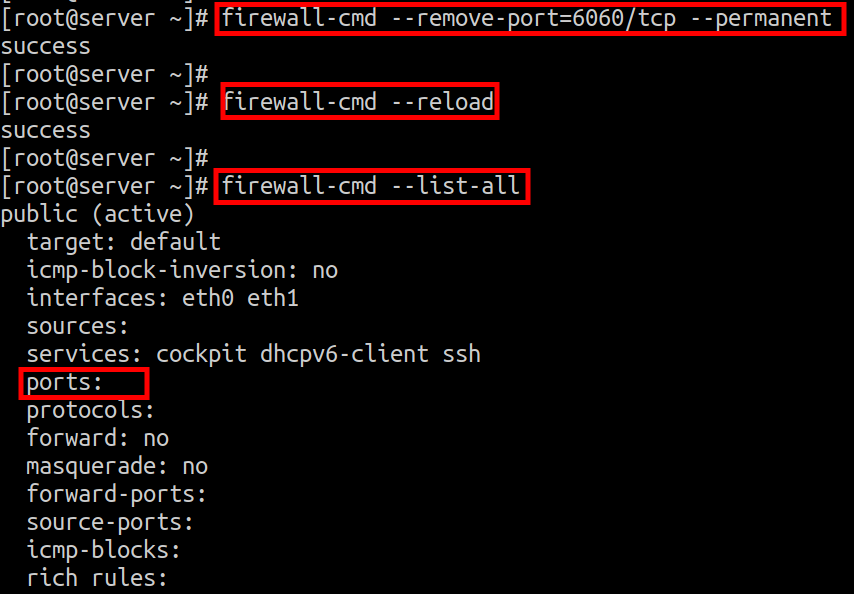
\includegraphics[scale=0.4]{content/chapter2/images/zones9.png}
			\caption{Sample output}
			\label{fig:zones9}
		\end{figure}
			
		
		
	\end{itemize}
	
\end{flushleft}
\newpage
